\documentclass{article}
\usepackage{graphicx}
\usepackage{geometry}
\usepackage{fancyhdr}										% Headers and footers
\usepackage{xcolor}											% Better colors
\usepackage{xpatch}											% Better macro patches
\usepackage{hyperref}										% Hyperlinks
\usepackage{fontspec}										% Custom fonts
\usepackage{tikz}											% Graphics creation
\usepackage{float}											% Figure positioning
\usepackage{tabu}											% Better tables
\usepackage[font={small,it}]{caption}						% Italic captions
\usepackage{listings}
\geometry{left=1in,right=1in,top=1in,bottom=1in}

\hypersetup{
	colorlinks=true,
	linkcolor=black
}

%************************************************%
\title{Lab 1 Report}
\author{Jinzhi Cai,Yifei Che, Ryan Anthony Kane}
\date{\today}
%************************************************%


\makeatletter
\begin{document}
\maketitle
\newpage
\tableofcontents
\clearpage
\section{Introduction}
Before beginning with the following experiments, we will first explore what board we will be using, the Beaglebone Green Wireless. A Beaglebone is a small, low-power open source computer capable of running different Linux flavors. When it comes to hardware, the Beaglebone Green Wireless has six main components shown in the table below.
\begin{table}[H]
	\centering
	\begin{tabu}{l | c }
		Component                                 & Functionality                                        \\ \hline
		Sitara AM3358BZCZ100                      & The main processor                                   \\\hline
		Micron 512MB DDR3L or Kingston 512mB DDR3 & The Dual Data Rate RAM memory                        \\\hline
		TPS65217C PMIC                            & Distributes the board power rails                    \\
		                                          & to various components on the board                   \\\hline
		SMSC Ethernet PHY                         & Physical network interface                           \\\hline
		Micron eMMC                               & Onboard MMC chip that holds up to 4GB of storage     \\\hline
		Wilink 8 Module                           & Adds Bluetooth and WLAN support on the 2.4 GHz range
	\end{tabu}
	\caption{Summary of Revision History}
	\label{tab:rev}
\end{table}
Now that we are familiar with the hardware that the board offers, we can continue to the remaining experiments.
\clearpage
\section{Download, Build an Image, and Boot the Beaglebone from an SD Card}
\subsection{Setup}
In the remainder of this lab, debian will be used on the Beaglebone. In order to run the latest debian image on the board, an SD card must be inserted into the board with the system image on it. The only setup for this experiment is having an SD card with a minimum of 4GB of storage on it.

\subsection{Procedure}
First, the latest system image can be obtained at https://beagleboard.org/latest-images. Here the system image downloaded is the “Debian X.X 4GB SD IoT”. While the LXQT images can also be installed, the beaglebone green wireless cannot take advantage of their GUI because it does not have an HDMI connection. After the image is downloaded, it has to be extracted from an .img.xz file to a .img file. After this is done, the image is then flashed to the SD card using Etcher. In Etcher select the SD Card, press flash and wait for the process to finish. Now, make sure the board is powered down by unplugging it from the computer if it is plugged in. Then insert the SD card and plug it back into the computer while holding the user button until it is booted successfully. 

\subsection{Result}
After the board is booted properly, it can be accessed via SSH from a terminal on the connected computer via USB. This can be done by running “ssh debian@192.168.6.2” or “ssh debian@192.168.7.2” depending on the system. If done properly, you will be prompted for a password, which by default is “temppwd”. This means the board is successfully booted off the SD card and we are ready to continue to the next experiment.
%---------------------1_1
\begin{center}
	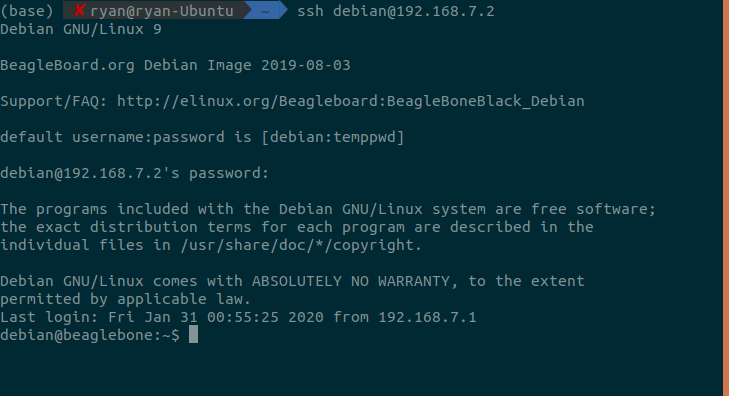
\includegraphics[width=0.8\textwidth]{img/Lab1_1.PNG}
\end{center}
\clearpage
\section{Copy the image to the eMMC and Boot the Beaglebone from the eMMC}
\subsection{Setup}
In this experiment, the system image on the SD card previously booted off of by the board will be flashed to the onboard eMMC so the SD card is no longer needed by the board. This can be avoided if you are fine with keeping that SD card in the Beaglebone permanently. No setup is required for this step.
\subsection{Procedure}
The first step to flash the system image to the eMMC is to SSH into the board while it is booted off of the SD card. Then, open the file uENV.txt in the /boot directory. Inside of the file, uncomment the line “cmdline=init=/opt/scripts/tools/eMMC-flasher-v3.sh”. This causes the SD card image to flash to the eMMC. Now, power down the board and reboot it while holding the user button until the LED sequence near the USB port lights up in such a way repetitively.
\begin{center}
	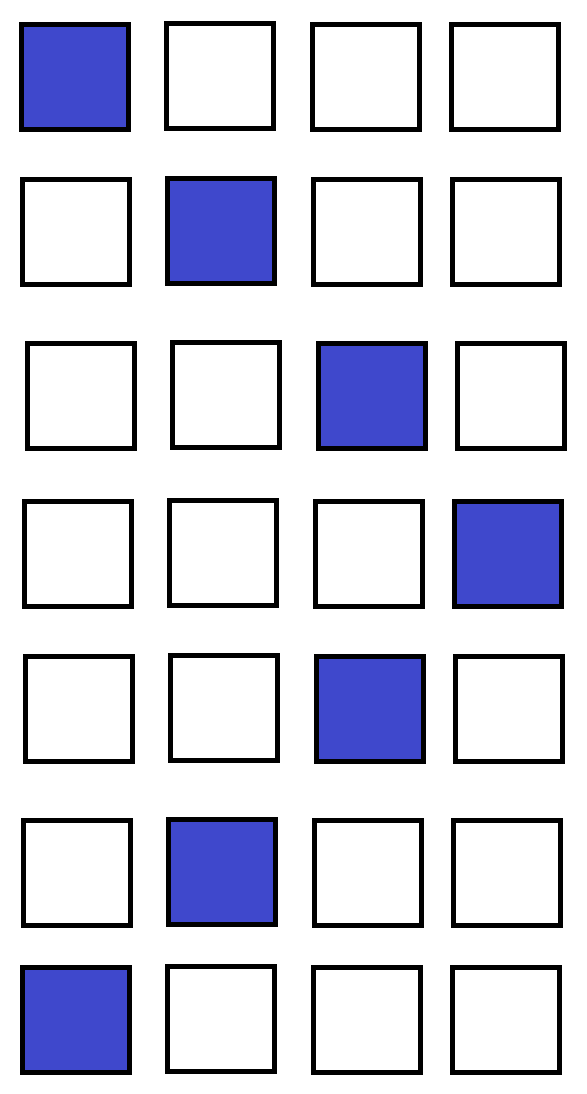
\includegraphics[width=0.2\textwidth]{img/Lab1_2.PNG}
\end{center}
Once the process is finished, the board will power down by itself. Finally, disconnect the board from the computer, remove the SD card and reconnect.
\subsection{Result}
After the board is rebooted, it can be accessed again via SSH from the computer terminal as done in the previous experiment. Congratulations the board now boots off of the onboard eMMC image!
%---------------------1_3
\begin{center}
	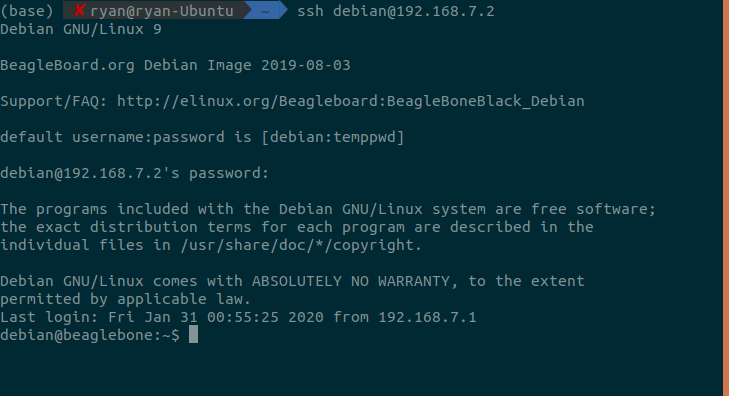
\includegraphics[width=0.6\textwidth]{img/Lab1_3.PNG}
\end{center}
\clearpage
\section{GPIO with the Beaglebone using the command line interface}
\subsection{Setup}
Now, in this experiment the Beaglebone GPIO ports will be controlled and tested using the terminal interface over SSH. To set up this experiment, the Analog Discovery was connected to a GPIO pin on the beaglebone. The pin diagram for the Beaglebone green wireless is shown below. Pin 0 of the Analog Discovery is connected to GPIO pin 48 of the Beaglebone and pin 1 on the Analog Discovery is connected to GPIO pin 49. Open staticIO in Waveforms so that the pin values can be seen.
%---------------------1_4
\begin{center}
	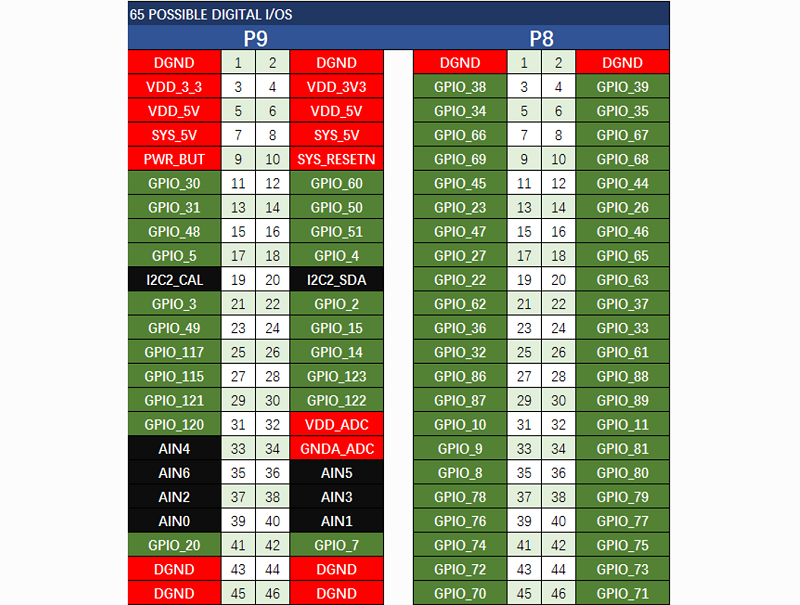
\includegraphics[width=0.8\textwidth]{img/Lab1_4.PNG}
\end{center}
\subsection{Procedure}
After SSHing into the Beaglebone, navigate to the /sys/class/gpio directory. Here the possible GPIO ports are shown as directories. To make sure pin 48 and 49 are available, run “export gpio48” and “export gpio49” in terminal. Now, navigate into the gpio48 directory. Inside of this directory there are two files that control the GPIO port. First, the direction of the pin can be set by writing in or out into the “direction” file. To set it as an output, execute “echo out > direction”. Now, running “echo 1 > value” sets the gpio pin to high, and 0 will set it to low. To read the value being sent by the Analog Discovery on pin 49, navigate up a directory level and into the gpio49 directory. Here, to set it as an input execute “echo in > direction” in terminal. After that, the value can be read using “cat value”.
\subsection{Result}
When gpio48/value is set to 1, the Analog Discovery pin 0 in staticIO reflects it, showing high, and vice versa for 0. Setting pin 1 on the Analog Discovery to low cause “cat value” in the gpio49 directory to be 0 and vice versa for high. This means we can correctly manipulate and read the Beaglebone GPIOs from the command line
\clearpage
\section{GPIO with the Beaglebone using C++ code}
\subsection{Setup}
Since we don’t always want to navigate to, read, and set pin values from the command line, C++ code will be developed to do this for us. This will let us programmatically operate the GPIO pins easier. The only setup required for this experiment is to connect two more GPIO pins to the analog discovery, and to make sure g++ is installed on the Beaglebone so the C++ code can be compiled into an executable.

\subsection{Procedure}
Writing this C++ code comes down to using file I/O to control the files used in the previous experiment. For this, fstreams are used to write and read the value and direction files. The full C++ class code can be found in Appendix A. After creating the C++ class it is implemented in the main.cpp file in order to setup two pins and inputs, and two as outputs. The input pins read the values sent from the Analog Discovery, and the values are reflected on the two pins set as outputs. The main.cpp file is shown below.
\begin{center}
	\begin{lstlisting}
#include "gpioHandle.h" 
#include <iostream> 
#include <cstdlib> 
#include <unistd.h> 


int main(){ 
	gpioHandle gpio; 
	int res; 
	res = gpio.initializePin(60,0,0); 
	res = gpio.initializePin(117,0,0); 
	res = gpio.initializePin(48,1,0); 
	res = gpio.initializePin(49,1,0); 
	
	int value;
	while(1) {
		value = gpio.getPinVal(48);
		gpio.setPinVal(60, value);
		value = gpio.getPinVal(49);
		gpio.setPinVal(117, value);
	}
} 
	\end{lstlisting}
\end{center}
\subsection{Result}
After the executable is run, the values set on the Analog Discovery are correctly reflected on the output pins of the board. This can be verified using staticIO in Waveforms.
\clearpage
\section{Test the speed of GPIO in Linux c++ using the flip-a-bit program }
\subsection{Setup}
We used the C++ code implemented for GPIO support in the previous section and add the feature to control the behavior of flip-a-bit program, then we used the analog discovery to monitor the outcome and frequency of the flip-a-bit. 
\subsection{Procedure}
We write a main program using our previously written GPIO class that runs a loop setting a GPIO output pin high and then low as fast as possible. Inside the code, we have the bit flipping between 0 and 1 in an infinite while loop. The program results in the Logic to produce a square wave at the output of the selected GPIO pin.
\subsection{Result}
In the analog discovery logic, we observe that the frequency of flip-a-bit is 5kHz. The reason why we get the 5kHz frequency instead of 1Ghz is that the time interval corresponds to how quickly the kernel of the OS is updated.
\begin{center}
	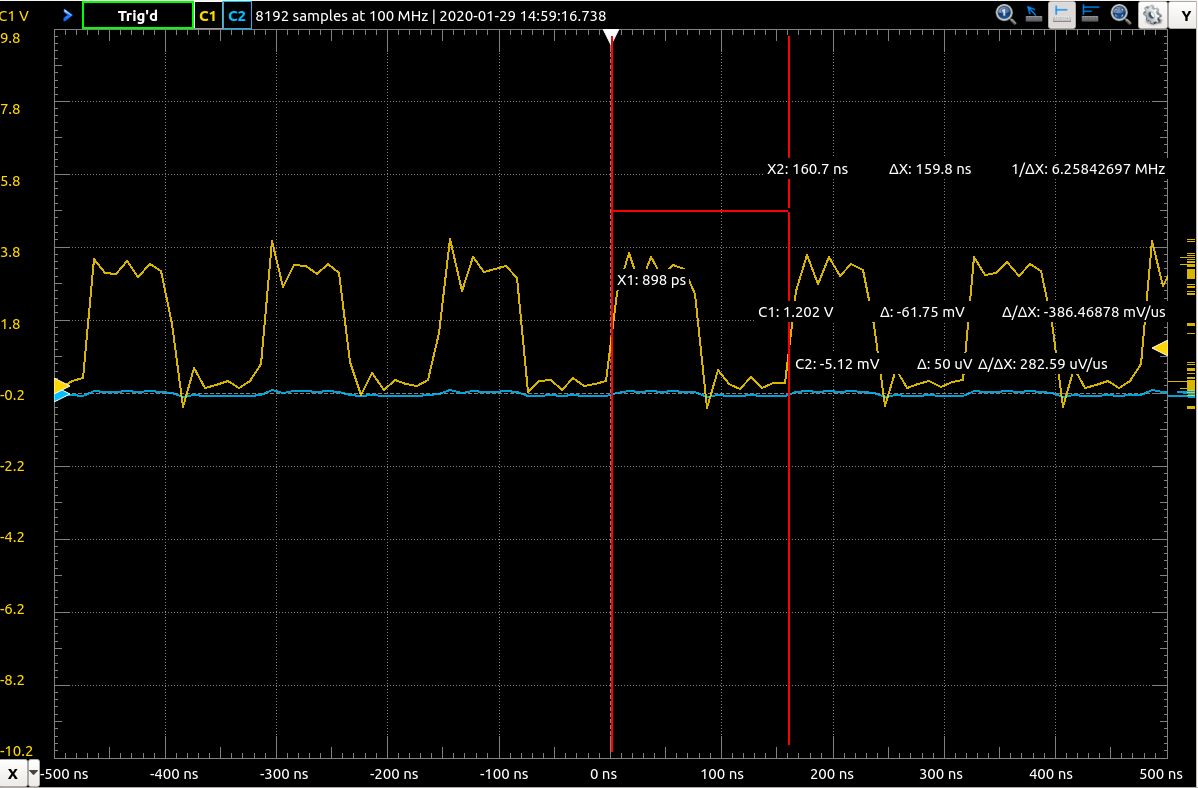
\includegraphics[width=0.8\textwidth]{img/Lab1_7.PNG}
\end{center}
\clearpage
\section{PWM with the Beaglebone using the command line interface}
\subsection{Setup}
Beaglebone has several PWM pins built inside the hardware, and we can connect the PWM pins. As soon as we finish connecting PWN pins, in order to control the PWM signals, we can use the command line interface to control the behavior. Later, we need to use type in command in the terminal to set the duty cycles, frequency, and period to control the value of PWMs. In the end, we need to use analog discovery to observe the duty cycle of the PWM.
\subsection{Procedure}
Firstly, we look at the Beaglebone Pinout Diagram to find the PWM pins. As the diagram indicates, each three PWMs are grouped as one, and two of them are a pair. We determine that we are going to use P9\_42 as our PWM pin. It’s located in the folder “/sys/class/pwm/pwm-1:0”. As we are in this directory, we type in the command “config-pin -q P9\_42” and “Config-pin -q P9\_42 pwm”, now, this pin is set up as a PWM pin. Then we can manually set the value of duty cycle, frequency, and period by echo values to those variables. The corresponding duty cycle is shown in the analog discovery. 
\subsection{Result}
After we set up the pin P9\_42 as a PWM pin, we manually set the duty cycle to 1000, 10000 to the period, now the duty cycle is 10\% since 1000/10000 is ten percent. About ten percent of each period is high, which shows the duty cycle of PWM observed in analog discovery. 
\begin{center}
	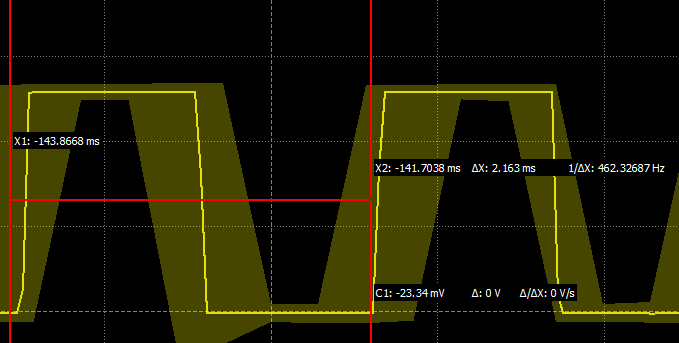
\includegraphics[width=0.8\textwidth]{img/Lab1_9.PNG}
\end{center}
\clearpage
\section{PWM with the Beaglebone using c++ code}
\subsection{Setup}
Beaglebone has several PWM pins built inside the hardware, and we can connect the PWM pins. As soon as we finish connecting PWN pins, in order to control the PWM signals, we need to use the C++ code to control the behavior. As the instruction indicates, we don’t have to configure the pins as PWM with code since we assume the pin is already configured as PWM by using the command line in the previous section. 
\subsection{Procedure}
Firstly, we need to construct a C++ code to control the PWM behavior of beaglebone. In the code, we define certain variables such as period, pinMode, etc. Then we determine we are going to use slot 21(1:1), 22(1:0) as our PWMs. In the code, the pwmHandle function contains the directories of these 3 PWMs and enable the pwm as well as assigns value to period for PWMs. ~pwnHnadle function disables the PWM. setPinVal function will set the value of duty cycle. 	In the main class, we pick PWM0, and inside an infinite while loop, we can increment the value of duty cycle. As soon as the duty cycle hits 100\%, it goes back to 0\% since "i\%=max".
\subsection{Result}
After compiling our C++ code, and execute the object file, we can observe that the duty cycle of the PWM is varying from 0\% to 100\% then back to 0\% in the waveform. 
\begin{lstlisting}
#ifndef PWM_HANDLE
#define PWM_HANDLE

#include <iostream>
#include <fstream>

using namespace std;

// pinmode definitions
#define PINMODE_OUT	0
#define PINMODE_IN	1
#define period 1000000
#define PWM0 0
#define PWM1 1
#define PWM2 2

class pwmHandle
{
	public:
	
	pwmHandle(int pin);
	~pwmHandle(); // unexport all pins opened by this class only
	int setPinVal(int duty_cycle_in); 
	// retuns -1 when pin is unusable, else returns 0
	
	private:
	string pwms[3][2]={{"P9_42","-0\:0"},{"P9_22","-1\:0"},{"P9_21","-1\:1"}};
	string name;
	ofstream duty_cycle;
	ofstream en;
	char *buffer;	// for sprintfs
	string path;
};

#endif
\end{lstlisting}
\begin{lstlisting}
#include "pwmHandler.h"
#include <cstring>
#include <unistd.h>
using namespace std;
pwmHandle::pwmHandle(int pin){
	std::string cmd(string("config-pin ")+pwms[pin][0]+string(" pwm"));
	system(cmd.c_str());
	path="/sys/class/pwm/pwm";
	path+=pwms[pin][1];
	ofstream pinMode;
	pinMode.open(path+"/period");
	pinMode << period << endl;
	pinMode.close();
	en.open(path+"/enable");
	en << "1" << endl;
	en.close();
	cout << path+"/enable" << endl;
}
pwmHandle::~pwmHandle(){
	duty_cycle.open(path+"/duty_cycle");
	en.open(path+"/enable");
	duty_cycle << "0"<< endl;
	en << "0"<< endl;
	duty_cycle.close();
	en.close();
}
int pwmHandle::setPinVal(int duty_cycle_in){
	char duty_cycle_value[21];
	sprintf(duty_cycle_value, "%d", duty_cycle_in);
	
	duty_cycle.open(path+"/duty_cycle");
	duty_cycle << duty_cycle_value<< endl;
	duty_cycle.close();
}
\end{lstlisting}
\clearpage
\section{ADC (Analog In) with the Beaglebone using the command line interface}
\subsection{Setup}
In this section we will use the ADC with BeagleBone to measure the voltage using a potentiometer.The BeagleBone has six ADC pins and six analog input pins. The maximum voltage of ADC pins is 1.8 Volts between GND\_ADC and VDD\_ADC.
We also need a 1 potentiometer we adjust voltage and several cables to connect the hardware. 
\subsection{Procedure}
The potentiometer has 3 terminals. The terminal 1 and 3 connect to the end points of GND\_ADC and VDD\_ADC. The second terminal is connected to the analog discovery pin. As the scroller scrolls, the resistance values across terminals 1 and 2 and terminals 2 and 3 change. Thus, the potentiometer acts like a voltage divider. 
\subsection{Result}
The value of the potentiometer is printed out in the terminal after we compile and run the file.
\begin{center}
	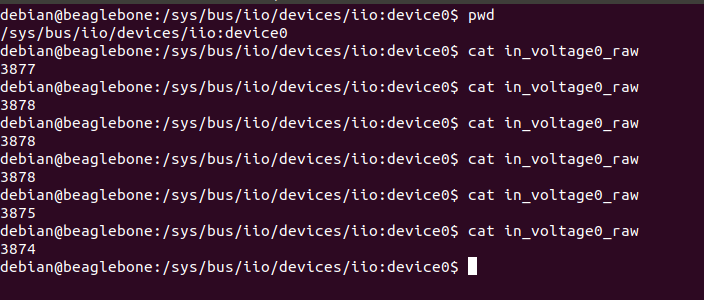
\includegraphics[width=0.8\textwidth]{img/Lab1_8.PNG}
\end{center}
\clearpage
\section{ADC (Analog In) with the Beaglebone using c++ code}
\subsection{Setup}
In this section we will use the ADC with BeagleBone to measure the voltage using a potentiometer.The BeagleBone has six ADC pins and six analog input pins. The maximum voltage of ADC pins is 1.8 Volts between GND\_ADC and VDD\_ADC.
We also need a 1 potentiometer we adjust voltage and several cables to connect the hardware. Moreover, this time we need to construct a C++ file to read the value from the ADC pin and print the value out in the terminal.
\subsection{Procedure}
We build our C++ code to take value form the ADC pin and print the value out in the terminal.
Basically, we construct the ADC class similar to the PWM class. Now the ADC class contains the functions "adcHandler", "~adcHandler", and "getPinVal". adcHandler will get the path of the ADC device. getPinVal will get the value of duty cycle. In the main class, we create an infinite while loop that keeps it running.
Then we can observe the ADC voltage value in the terminal after we compile and run the file. By scrolling the spin of the potentiometer, we can see the value varies. 
\subsection{Result}
Then the value printed out will be manually countrolled by the spin. 
\begin{lstlisting}
#ifndef ADC_HANDLE
#define ADC_HANDLE

#include <iostream>
#include <fstream>

#define ADC_PATH "/sys/bus/iio/devices/iio:device0/in_voltage%d_raw"

using namespace std;
class adcHandle
{
	public:
		adcHandle(int device);
		~adcHandle(); // unexport all pins opened by this class only
		int getPinVal(); // retuns -1 when pin is unusable, else returns 0
	
	private:
		string path;
};

#endif
\end{lstlisting}
\begin{lstlisting}
#include "adcHandler.h"
using namespace std;
adcHandle::adcHandle(int device){
	if (device>7)return;
	char char_path[55];
	sprintf(char_path, ADC_PATH, device);
	path=char_path;
}
adcHandle::~adcHandle(){

} // unexport all pins opened by this class only
int adcHandle::getPinVal(){
	ifstream getVal;
	getVal.open(path);
	int result =0;
	getVal >> result;
	getVal.close();
	return result;
} // retuns -1 when pin is unusable, else returns 0
\end{lstlisting}
\clearpage
\section{Embedded System}
\subsection{Setup}
In this section,we use all the class we made in the previous lab to create a embedded system that can react base on the input form the ADC and present the result in the screen and the LED light.
The whole lab contain three component. The connection is in following form.
\begin{center}
	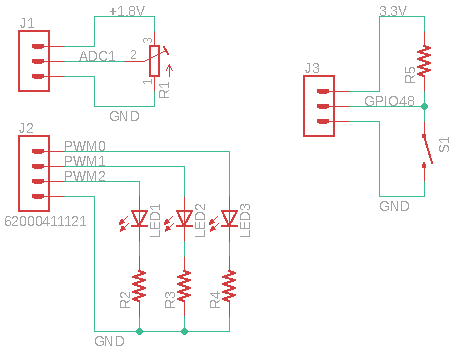
\includegraphics[width=0.5\textwidth]{img/Lab1_5.PNG}
\end{center}
\subsection{Procedure}
Connecting the circuit base on the image. The program contain three region. The first region is set up. The purpose for this region is to set up all the peripheral require in the program. The second region and the third region all contain in the while loop. The second region is to write the value to the PWM module and the third region is use to read the value from the ADC and save to selected channel.
\subsection{Result}
Even though the brightness for each channel is different which is due to the characteristic of different color LED, it still will be able to get the different brightness for different channel base on the ADC value.
\begin{center}
	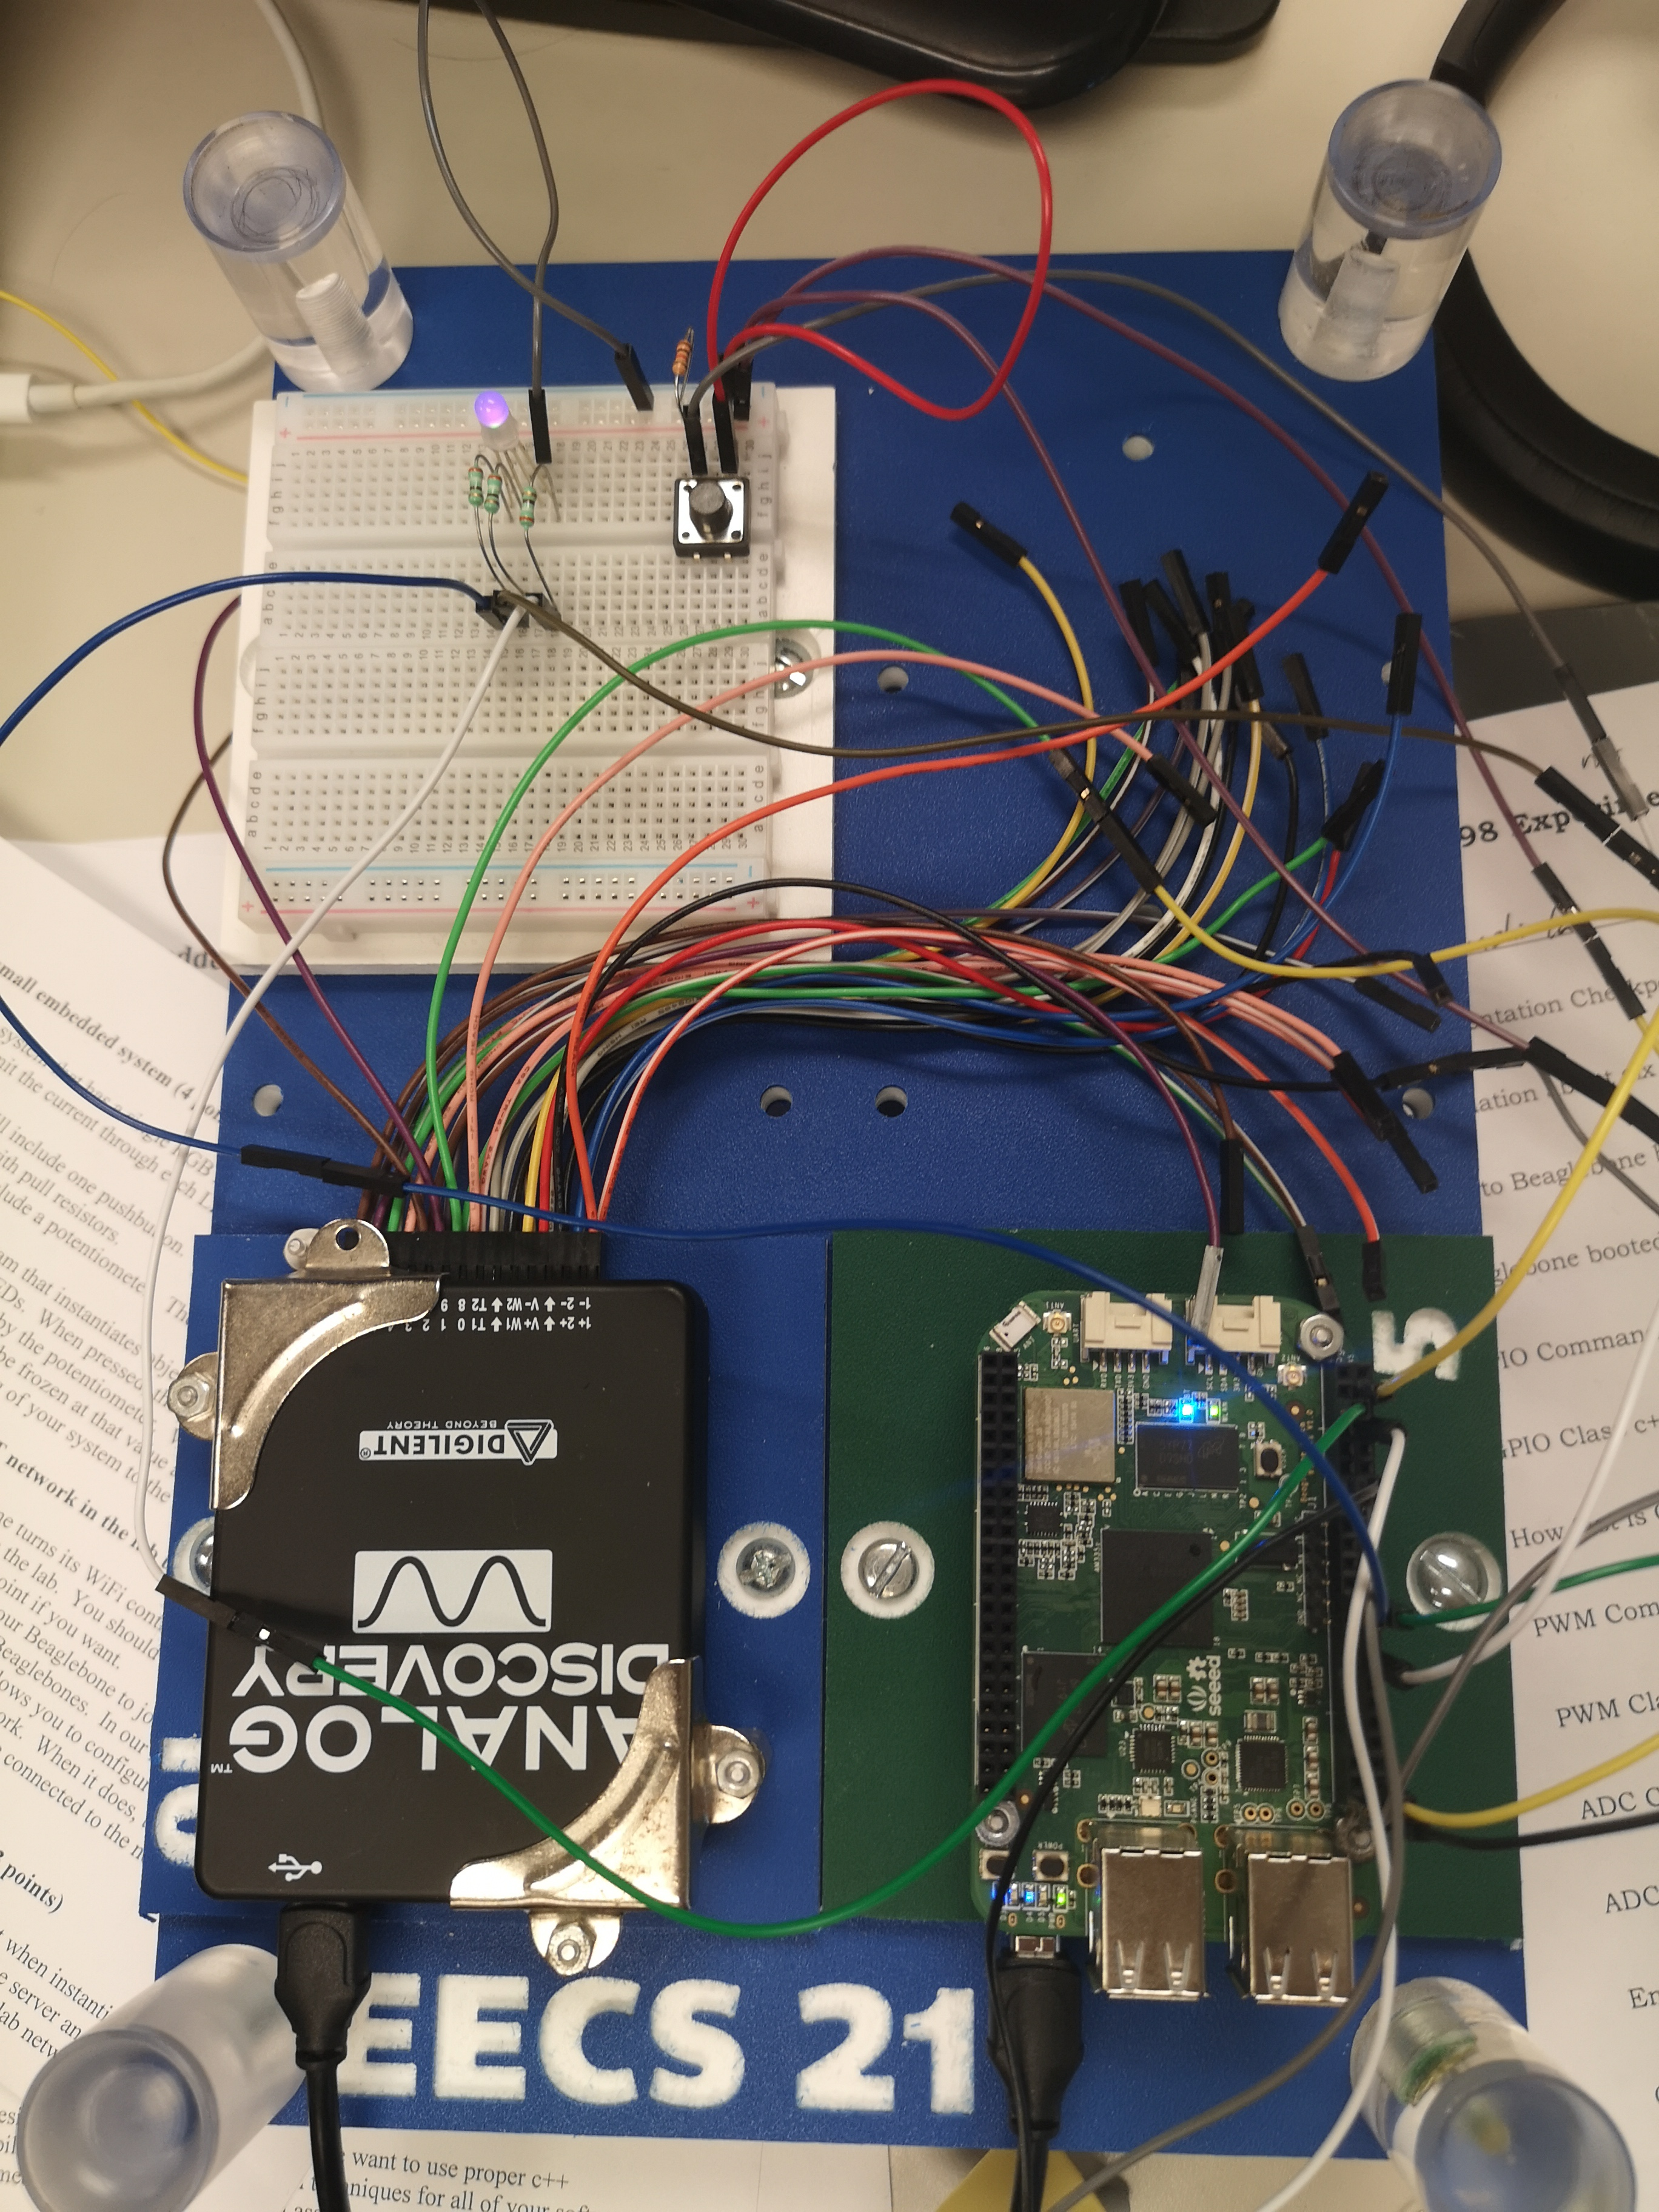
\includegraphics[width=0.3\textwidth]{img/Lab1_6.jpg}
\end{center}
\clearpage
\section{Connection to iot\_lab network}
\subsection{Setup}
In this section, we will use the connmanctl to make the beaglebone connect to the iot\_lab wifi network. The requirement for this lab is following.
\begin{itemize}
	\item Beaglebone Green
	\item Connmanctl
	\item Working wifi router
\end{itemize}
\subsection{Procedure}
\begin{itemize}
	\item  Open connmanctl\\>> \$ connmanctl 
	\item Scan wifi \\>> connman\$ scan wifi 
	\item Check services avaliable \\>> connman\$ services \\lot\_lab wifi\_dc85de828967\_38303944616e69656c73\_managed\_psk  
	\item Start agent \\>> connman\$ agent on 
	\item Connect to the WIFI \\>> connman\$ connect  wifi\_dc85de828967\_38303944616e69656c73\_managed\_ps 
	\item Key in the password \\Agent RequestInput wifi\_dc85de828967\_38303944616e69656c73\_managed\_psk \\Passphrase = [ Type=psk, Requirement=mandatory ] \\Passphrase?  
	\item Ifconfig check connection \\>> \$ ifconfig 
\end{itemize}
\subsection{Result}
After type the ifconfig....
\begin{lstlisting}
wlan0: flags=4163<UP,BROADCAST,RUNNING,MULTICAST>  mtu 1500
	inet 10.2.19.112  netmask 255.255.224.0  broadcast 10.2.31.255
	inet6 fe80::52ee:62b2:c8ce:7be8  prefixlen 64  scopeid 0x20<link>
	ether d4:25:8b:dd:3a:bf  txqueuelen 1000  (Ethernet)
	RX packets 105  bytes 6602
	RX errors 0  dropped 0  overruns 0  frame 0
	TX packets 560  bytes 402
	TX errors 0  dropped 0 overruns 0  carrier 0  collisions 0
\end{lstlisting}
\clearpage
\section{Sending Data Over a Socket}
\subsection{Setup}
In this section, we will use the TCP socket to make the beaglebone connect to the laptop via wifi network. The requirement for this lab is following.
\begin{itemize}
	\item Beaglebone Green
	\item Working wifi router
\end{itemize}
\subsection{Procedure}
The server program contain two parts. The server handler is opening a listen port on the network socket. It also help the main class to transmit and receive the data. The main class is to read in the data that get from the TCP connection and send information back to the client.
\begin{lstlisting}
	Server foo(9090);
	foo.listen();
	std::cout<<"Got \"";
	std::cout<<foo.receive(12);
	std::cout<<"\" from the client\n";
	std::cout<<"Sending \"Hello Client\" to the client\n";
	foo.send("Hello Client");
\end{lstlisting}
\subsection{Result}
After execute this program in the, client is netcat. Connect to the server and it do reply the the welcome message. 
\clearpage
\section{Conclusion}
Embedded system is also a improtant part in the people's life. By running this lab, we understand the basic structure for a embedded system. The system we design, even it is very simple, but can apply to many different area. As the computer system that the most close the physical world, a lot of the debugging work is not only in the software layer. It create new challenge to the engineers to uncover a system that have problem.
\section{Appendix A: C++ Gpio Class Code}
\begin{center}
	\begin{lstlisting}
#include "gpioHandle.h" 
#include <cstring> 
#include <unistd.h> 


gpioHandle::gpioHandle() 
{ 
} 


gpioHandle::~gpioHandle() 
{ 
} 


//exports pin and sets mode 
int gpioHandle::initializePin(const int pin, const int mode, const bool  initialValue) { 
	char pinNum[21]; 
	std::string fordirection("/direction"); 
	std::string path("/sys/class/gpio/gpio"); 
	sprintf(pinNum, "%d", pin); 
	path += pinNum; 
	ofstream exportPin; 
	exportPin.open("/sys/class/gpio/export"); 
	if(!exportPin.is_open()) { 
		cout << "Error! exportPin not open. \n"; 
		return (-1); 
	} 
	exportPin << pin; 
	exportPin.close(); 
	
	
	path += fordirection;   
	usleep(100000); 
	ofstream pinMode; 
	pinMode.open(path); 
	if(!pinMode.is_open()) { 
		cout << "Error! pinMode not open \n"; 
		return (-1); 
	} 
	if (PINMODE_OUT == mode) { 
		pinMode << "out"; 
	} else { 
		if (PINMODE_IN == mode) { 
			pinMode << "in"; 
		} else { 
			cout << "ERROR!!! \n"; 
			return (-1); 
		} 
	} 
	pinMode.close(); 
	usleep(100000); 
	// cout << "Pin " << pin << " initialized to mode "; //debug only 
	switch(mode){ 
		case(PINMODE_OUT): 
		cout << "OUTPUT"; break; 
		case(PINMODE_IN): 
		cout << "INPUT"; break; 
		default: 
		cout << "INVALID PINMODE"; break; 
	} 
	cout << " with an intial value of " << initialValue << endl; 
	return(0); 
} 


// changes pin mode 
int gpioHandle::setPinMode(const int pin, const int mode, const bool initialValue) { 
	char pinNum[21]; 
	std::string fordirection("/direction"); 
	std::string path("/sys/class/gpio/gpio"); 
	sprintf(pinNum, "%d", pin); 
	path += pinNum; 
	path += fordirection; 
	ofstream pinMode; 
	pinMode.open(path); 
	if(!pinMode.is_open()) { 
		cout << "Error! \n"; 
		return (-1); 
	} 
	
	if (PINMODE_OUT == mode) { 
		pinMode << "out"; 
	} else { 
		if (PINMODE_IN == mode) { 
			pinMode << "in"; 
		} else {  
			cout << "ERROR!!! \n"; 
			return (-1); 
		} 
	} 
	pinMode.close(); 
	
	
	usleep(100000); 
	// cout << "Pin " << pin << " set to mode "; //debug only 
	switch(mode){ 
		case(PINMODE_OUT): 
		cout << "OUTPUT"; break; 
		case(PINMODE_IN): 
		cout << "INPUT"; break; 
		default: 
		cout << "INVALID PINMODE"; break; 
	} 
	// cout << " with an intial value of " << mode << endl; 
	return(0); 
} 

// retuns -1 when pin is unusable, else returns 0 
int gpioHandle::setPinVal(const int pin, const bool val) { 
	char pinNum[21]; 
	std::string forvalue("/value"); 
	std::string path("/sys/class/gpio/gpio");; 
	sprintf(pinNum, "%d", pin); 
	path += pinNum; 
	path += forvalue; 
	fstream setVal; 
	setVal.open(path); 
	if(!setVal.is_open()) { 
		cout << "Error! \n"; 
		return (-1); 
	} 
	
	
	// cout << "value is: " << (int)val << " Non cast: " << val << endl; 
	setVal << val; 
	// cout << "Pin " << pin << " set to " << val << endl;// debug only 
	setVal.close(); 
	usleep(100000); 
	return(0); 
} 

// returns -1 when pin is unusable, else retuns value 
int gpioHandle::getPinVal(const int pin){ 
	char pinNum[21]; 
	std::string forvalue("/value"); 
	std::string path("/sys/class/gpio/gpio"); 
	sprintf(pinNum, "%d", pin); 
	path += pinNum; 
	path += forvalue; 
	ifstream getVal; 
	getVal.open(path); 
	if(!getVal.is_open()) { 
		cout << "Error! \n"; 
		return (-1); 
	} 
	int value; 
	getVal >> value; 
	getVal.close(); 
	usleep(100000); 
	return(value); 
} 

// returns true if pin is usable 
bool gpioHandle::pinOpen(const int pin) { 
	char pinNum[21]; 
	std::string path("/sys/class/gpio/gpio"); 
	sprintf(pinNum, "%d", pin); 
	path += pinNum; 
	ofstream usePin; 
	usePin.open(path); 
	if(usePin.is_open()) { 
		cout << "The pin " << pin << " is usable!"; 
		return (true); 
	} else { 
		cout << "The pin " << pin << " is unusable!"; 
		return(false); 
	} 
	usePin.close(); 
	usleep(100000); 
	// cout << "Pin " << pin << " opened!" << endl; // debug only 
} 

// unexports pin 
int gpioHandle::pinClose(const int pin) { 
	char pinNum[21]; 
	int pinNumber = pin; 
	std::string path("/sys/class/gpio/gpio"); 
	sprintf(pinNum, "%d", pin); 
	path += pinNum; 
	ofstream unexportPin; 
	unexportPin.open("/sys/class/gpio/unexport"); 
	if(!unexportPin.is_open()) { 
		cout << "Error! \n"; 
		return (-1); 
	} 
	unexportPin << pinNumber; 
	unexportPin.close(); 
	// cout << "Pin " << pin << " closed!" << endl; // debug only 
	usleep(100000); 
	return(0); 
} 

	\end{lstlisting}
\end{center}
\end{document}